\documentclass{article}[18pt]
\ProvidesPackage{format}
%Page setup
\usepackage[utf8]{inputenc}
\usepackage[margin=0.7in]{geometry}
\usepackage{parselines} 
\usepackage[english]{babel}
\usepackage{fancyhdr}
\usepackage{titlesec}
\hyphenpenalty=10000

\pagestyle{fancy}
\fancyhf{}
\rhead{Sam Robbins}
\rfoot{Page \thepage}

%Characters
\usepackage{amsmath}
\usepackage{amssymb}
\usepackage{gensymb}
\newcommand{\R}{\mathbb{R}}

%Diagrams
\usepackage{pgfplots}
\usepackage{graphicx}
\usepackage{tabularx}
\usepackage{relsize}
\pgfplotsset{width=10cm,compat=1.9}
\usepackage{float}

%Length Setting
\titlespacing\section{0pt}{14pt plus 4pt minus 2pt}{0pt plus 2pt minus 2pt}
\newlength\tindent
\setlength{\tindent}{\parindent}
\setlength{\parindent}{0pt}
\renewcommand{\indent}{\hspace*{\tindent}}

%Programming Font
\usepackage{courier}
\usepackage{listings}
\usepackage{pxfonts}

%Lists
\usepackage{enumerate}
\usepackage{enumitem}

% Networks Macro
\usepackage{tikz}


% Commands for files converted using pandoc
\providecommand{\tightlist}{%
	\setlength{\itemsep}{0pt}\setlength{\parskip}{0pt}}
\usepackage{hyperref}

% Get nice commands for floor and ceil
\usepackage{mathtools}
\DeclarePairedDelimiter{\ceil}{\lceil}{\rceil}
\DeclarePairedDelimiter{\floor}{\lfloor}{\rfloor}

% Allow itemize to go up to 20 levels deep (just change the number if you need more you madman)
\usepackage{enumitem}
\setlistdepth{20}
\renewlist{itemize}{itemize}{20}

% initially, use dots for all levels
\setlist[itemize]{label=$\cdot$}

% customize the first 3 levels
\setlist[itemize,1]{label=\textbullet}
\setlist[itemize,2]{label=--}
\setlist[itemize,3]{label=*}

% Definition and Important Stuff
% Important stuff
\usepackage[framemethod=TikZ]{mdframed}

\newcounter{theo}[section]\setcounter{theo}{0}
\renewcommand{\thetheo}{\arabic{section}.\arabic{theo}}
\newenvironment{important}[1][]{%
	\refstepcounter{theo}%
	\ifstrempty{#1}%
	{\mdfsetup{%
			frametitle={%
				\tikz[baseline=(current bounding box.east),outer sep=0pt]
				\node[anchor=east,rectangle,fill=red!50]
				{\strut Important};}}
	}%
	{\mdfsetup{%
			frametitle={%
				\tikz[baseline=(current bounding box.east),outer sep=0pt]
				\node[anchor=east,rectangle,fill=red!50]
				{\strut Important:~#1};}}%
	}%
	\mdfsetup{innertopmargin=10pt,linecolor=red!50,%
		linewidth=2pt,topline=true,%
		frametitleaboveskip=\dimexpr-\ht\strutbox\relax
	}
	\begin{mdframed}[]\relax%
		\centering
		}{\end{mdframed}}



\newcounter{lem}[section]\setcounter{lem}{0}
\renewcommand{\thelem}{\arabic{section}.\arabic{lem}}
\newenvironment{defin}[1][]{%
	\refstepcounter{lem}%
	\ifstrempty{#1}%
	{\mdfsetup{%
			frametitle={%
				\tikz[baseline=(current bounding box.east),outer sep=0pt]
				\node[anchor=east,rectangle,fill=blue!20]
				{\strut Definition};}}
	}%
	{\mdfsetup{%
			frametitle={%
				\tikz[baseline=(current bounding box.east),outer sep=0pt]
				\node[anchor=east,rectangle,fill=blue!20]
				{\strut Definition:~#1};}}%
	}%
	\mdfsetup{innertopmargin=10pt,linecolor=blue!20,%
		linewidth=2pt,topline=true,%
		frametitleaboveskip=\dimexpr-\ht\strutbox\relax
	}
	\begin{mdframed}[]\relax%
		\centering
		}{\end{mdframed}}
\lhead{Computer Systems - Dr Magnus Bordewich}


\begin{document}
\begin{center}
\underline{\huge CPU Architecture}
\end{center}
\section{Components of a CPU}
\begin{center}
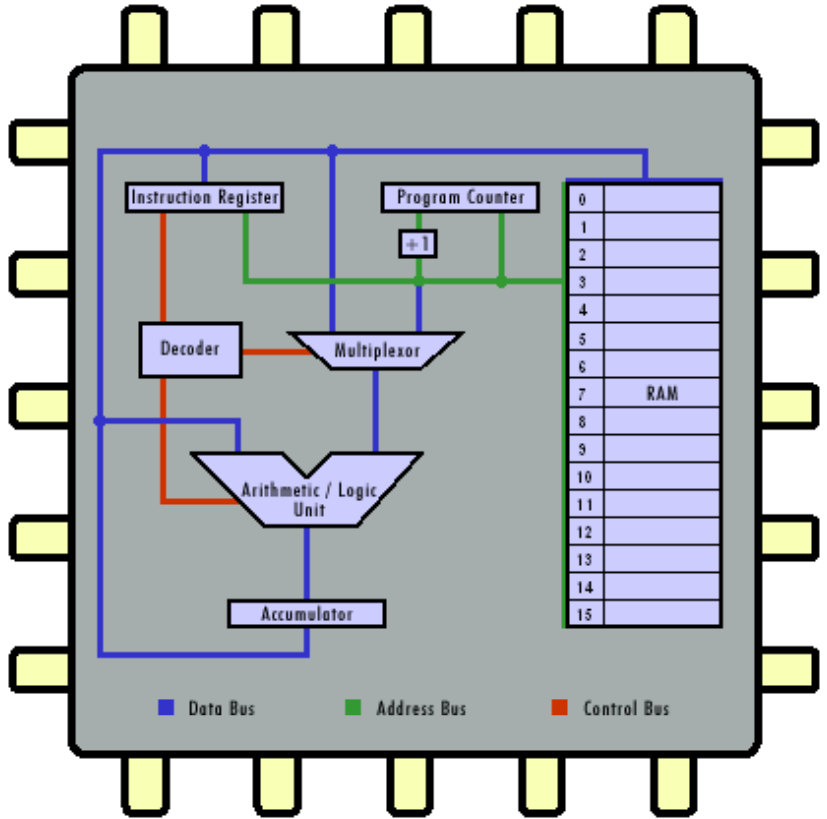
\includegraphics[width=6cm]{cpu_components.jpg}
\end{center}
5 major components
\begin{itemize}
\item \textbf{Memory} - RAM - "the mailboxes"
\item \textbf{Registers} - The special memory locations that can be accessed very fast. 3 registers are shown: the Instruction register (IR), the Program Counter (PC) and the Accumulator
\item \textbf{Arithmetic/Logic Unit} - "the calculator"
\item \textbf{Buses} - bundles of tiny wires that carry data between components. The three most important buses are the address,data and control buses
\item \textbf{Control Unit} - Responsible for directing the flow of instructions and data within the CPU
\end{itemize}
In the diagram the Decoder and Multiplexor comprise the Control Unit
\section{Registers}
"Work space" of the CPU\\
Storage locations in the CPU, often with a defined purpose and wired to perform that purpose\\
Hold a binary value for
\begin{itemize}
\item Storage
\item Manipulation
\item Calculation
\end{itemize}
Manipulated directly by the Control Unit\\
Vary in size from 1 to 128 bits
\subsection{Accumulator}
This is considered part of the ALU\\
These are general purpose registers used for:
\begin{itemize}
\item Holding data
\item Holding interim and final results of arithmetic operations
\item Holding data waiting to be transferred between different memory locations
\item Holding data waiting to be transferred between I/O and memory
\end{itemize}
\subsection{Registers in the Control Unit}
\subsubsection{Program Counter}
Holds the address of the next instruction to be executed
\subsubsection{Instruction Register (IR)}
Holds the actual instruction being executed
\subsubsection{Flags}
1 bit registers used to keep track of special conditions e.g. Arithmetic Carry, Overflow\\
Flags are grouped together into one or more status registers (SR)
\subsection{Memory management}
\subsubsection{Memory Address Register}
Holds the address of a memory location to be accessed, always written to, never from\\
Hardwired with an address bus to the ram, activate it to get the correct data
\subsubsection{Memory Data Register}
Holds the value that is being stored to or retrieved from the memory location currently addressed by the MAR\\
May be written to or from\\
Also known as the Memory Buffer Register
\section{Buses}

Bus - A physical connection that makes it possible to transfer data from one location in a system to another is called a bus\\
A bus is a group of electrical conductors (\textbf{lines}) used to carry signals
\begin{itemize}
\item \textbf{Data Bus} - Transfer Data
\item \textbf{Control Bus} - Controls what bits of circuitry are active
\item \textbf{Address Bus} - Activates the right part of the RAM to get data out of
\item \textbf{Power Bus} - Feed power to all parts of the chip
\end{itemize}
\subsection{Point-to-point}
Bus carries the signal from a specific source to a specific destination e.g. Home PC to Printer
\subsection{Broadcast}
Bus used to carry signals to many different devices
\subsection{Bus Interface Bridges}
Allows communications between the different buses, for example USB or PCIe
\end{document}